\apendice{Documentación técnica de programación}

\section{Introducción}
En este apartado se documentan todos los aspectos importantes para el proceso de programación.

\section{Estructura de directorios}
Este proyecto tiene una estructura de directorios propia de una aplicación Spring Boot MVC \cite{estructura-mvc}, en la que se pueden diferenciar los 3 componentes básicos del patrón Modelo-Vista-Controlador \ref{fig:estructura-elearningqa}.
\begin{figure}[H]
    \centering
    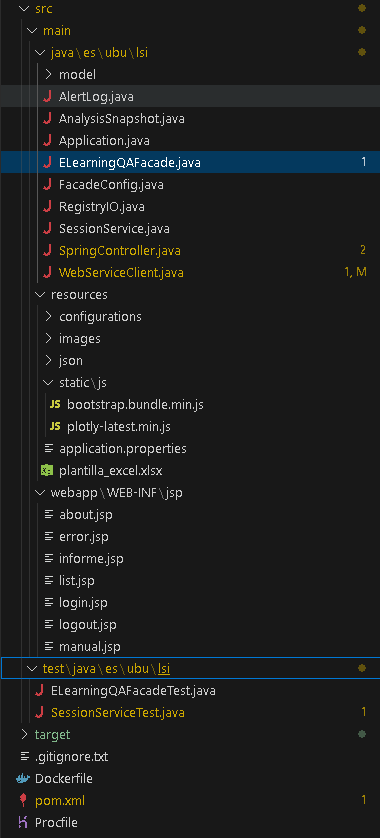
\includegraphics[width=0.6\linewidth]{img/estructura-proyecto.png}
    \caption{Estructura de proyecto de eLearningQA}
    \label{fig:estructura-elearningqa}
\end{figure}

\section{Manual del programador}
Este proyecto está construido con Spring Boot 2.7.18 como framework de desarrollo. Se utiliza Java JDK 8 que se puede descargar de la página oficial \cite{java8}. Para poder desarrollar en este proyecto también se necesita una versión de Apache Maven, la versión utilizada para este desarrollo ha sido la 3.9.6.

El IDE utilizado en este caso ha sido Visual Studio Code, se pueden utilizar otros IDE, el más recomendado para el desarrollo en java es IntelliJ IDEA. 

Para obtener el proyecto se puede acceder al repositorio en GitHub \cite{repositorio}. Hay varias formas de descargar el repositorio, una de ellas es utilizando el comando: 

\begin{verbatim}
git -clone https://github.com/bae1001/eLearningQA
\end{verbatim}

Además, el proyecto cuenta con integración continua con ``Java CI with Maven'', que se utiliza para hacer una comprobación de cada subida al repositorio para verificar que los cambios funcionan correctamente con el conjunto de la aplicación. Para esto existe un fichero de configuración llamado ``maven.yml'' situado en la carpeta de workflows de Github \ref{fig:mvn-ci}.

\begin{figure}[H]
    \centering
    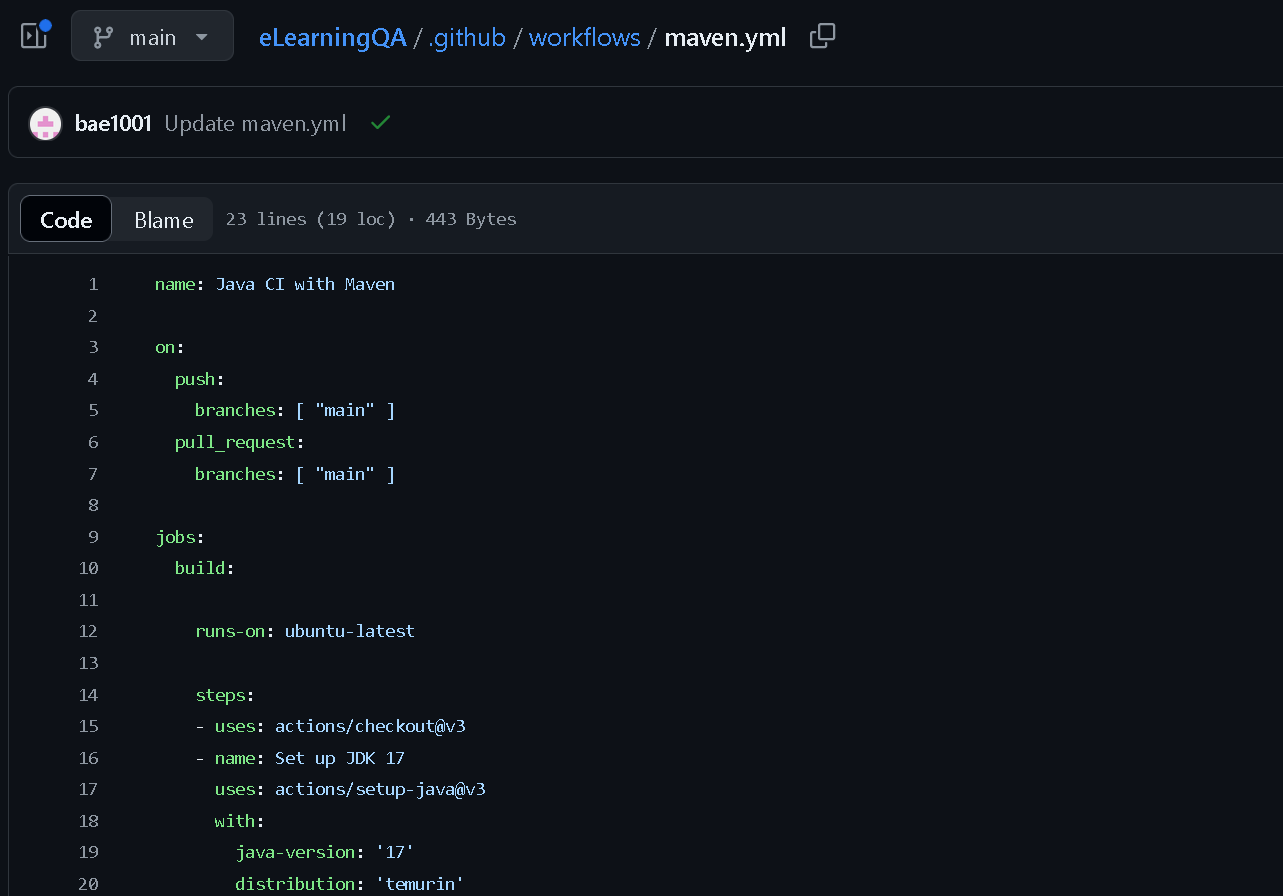
\includegraphics[width=1\linewidth]{img/javaCi_github.png}
    \caption{Fichero de configuración de Java CI with Maven en Github}
    \label{fig:mvn-ci}
\end{figure}

Por otro lado, es necesario disponer de Docker Desktop \cite{docker}, para poder hacer un despliegue en contenedores.

Finalmente, hay que configurar el fichero para la conexión con SonarCloud. Al igual que ``Java CI with Maven'' se debe configurar un fichero en la carpeta de workflows de Github, en este proyecto dicho fichero se llama ``build.yml'' \ref{fig:sonar-workflow}.
\begin{figure}[H]
    \centering
    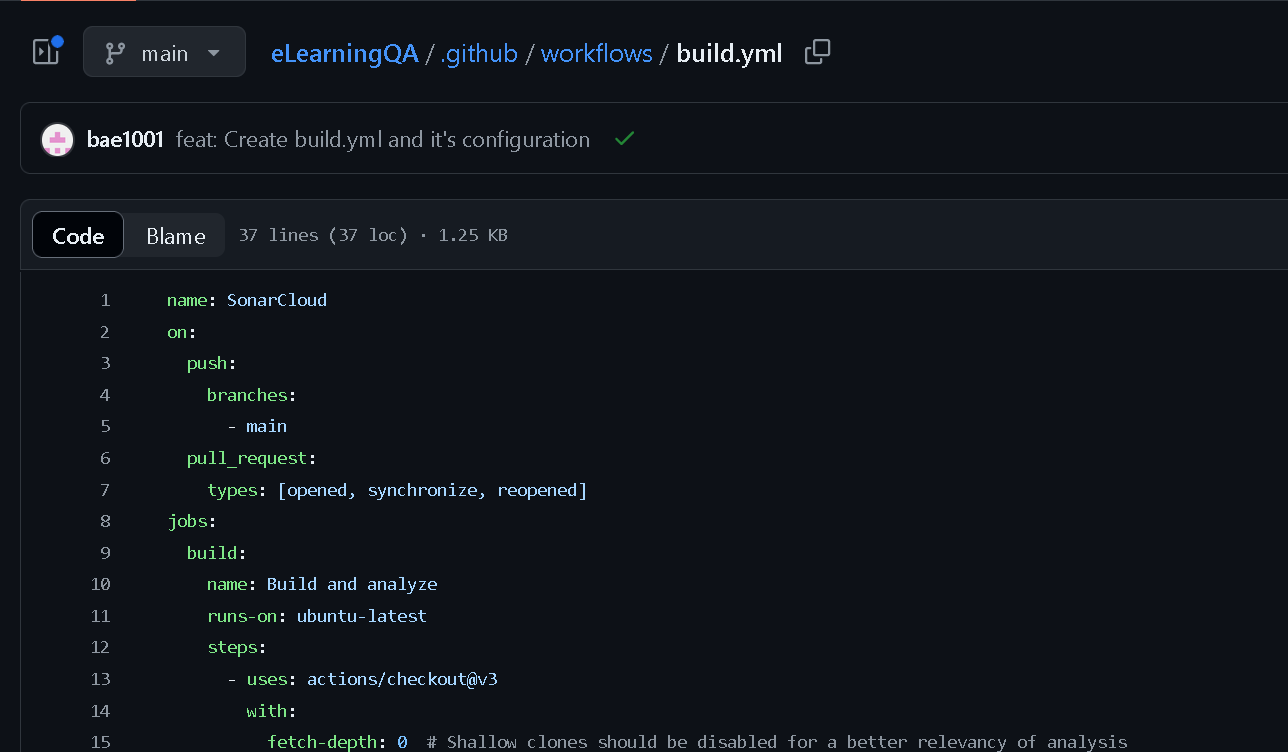
\includegraphics[width=1\linewidth]{img/sonar-workflow.png}
    \caption{Fichero de configuración de Sonarcloud en workflows de Github}
    \label{fig:sonar-workflow}
\end{figure}

\section{Compilación, instalación y ejecución del proyecto}
Para poder ejecutar este proyecto se deben seguir los siguientes pasos:
\begin{enumerate}
    \item Ejecutar el comando de compilación de Maven, a la altura del archivo pom del proyecto:
        \begin{verbatim}
            mvn clean install
        \end{verbatim}
    \item A continuación hay 3 opciones para poner en ejecución el proyecto:
        \begin{enumerate}
            \item Ejecutando el maín situado en la clase Aplication.java situada en el paquete src/main/java/es/ubu/lsi
            \item Ejecutando el .war generado en la compilación:
                \begin{verbatim}
                    java -jar prototipo-0.4-SNAPSHOT.war
                \end{verbatim}
            \item Ejecutando el proyecto en un contenedor de Docker. para ello lo primero será crear la imagen con el siguiente comando:
                \begin{verbatim}
                    docker build -t <nombreDeImagen> .
                \end{verbatim}
            A continuación, se ejecuta la imagen creada con el siguiente comando:
                \begin{verbatim}
                    docker run -p 8080:8080 <nombreDeImagen>
                \end{verbatim}
        \end{enumerate}
        \item A continuación se podrá acceder a la aplicación en localhost en la siguiente dirección:
        \begin{verbatim}
            http://localhost:8080/
        \end{verbatim}
\end{enumerate}


\section{Pruebas del sistema}
Para asegurar la mantenibilidad del proyecto es necesario tener test que aseguren el funcionamiento de las funcionalidades con el paso del tiempo y cuando se modifique código que afecte a dichas funcionalidades. Es una práctica muy recomendable en la calidad de código y conveniente para el desarrollo a largo plazo. Esta aplicación cuenta con test que prueban las funcionalidades principales del proyecto. Estos test se puede encontrar en la carpeta de test del proyecto y se pueden ejecutar manualmente o con el comando de compilación de Maven. 

Estas pruebas utilizan datos de prueba que se encuentran en \textbf{src/main/resources/json}, estos datos se han creado con el fin de cubrir la mayor cantidad de código posible.
